\chapter{Theory: The Basics}

Over the last decades, quantum chemistry has emerged as a crucial tool for investigating a wide variety of problems in chemistry. This, in combination with the increasing performance and widespread use of computers, has spawned a whole new branch of chemistry known as \emph{computational chemistry}. The field of computational chemistry uses methods developed in \emph{theoretical chemistry} and incorporates them into efficient programs. , quantum chemical methods are routinely applied to assist in solving problems related to chemical structure, reactivity and spectroscopy. However, one of the main problems in computational chemistry is choosing a suitable level of theory for a given problem - the best choice is always a trade-off between speed and accuracy, and requires intricate knowledge of the methods' theoretical and computational limits. This chapter summarizes the core concepts of quantum chemistry and its most important methods. It is by no means complete, and the reader is referred to the original text book resources for more details \cite{Sza1996,Hel2000,Jen2017,Nor2018,Sch2018}.

\section{Describing Dynamics in a Molecular System}

In order to describe a molecular system, one needs to decide
\begin{itemize}
\item what the fundamental particles are
\item what forces are governing them
\item what the starting conditions are
\item and what form the dynamical equations take.
\end{itemize}
\noindent The choice of particles dictates what properties the model is ultimately able to describe. For example, force field methods use atoms as the indivisible unit, which is sufficient to describe the molecular structure and dynamics of large molecules such as proteins, but does not provide any information on electron distribution. Using electrons and nuclei as the fundamental particles allows to get a better picture of the electron density and how it reacts to external perturbation, which is important for studies on reactivity and spectroscopic constants. To describe radioactive decay, it is necessary to further divide the nucleus into protons and neutrons. 

Smaller subdivisions lead to a stricter limit on the size of molecules that can be treated. Force field methods may describe the dynamics of molecules with several tens of thousands of atoms, while a finer grained method involving electrons can often only describe molecules one to two orders of magnitudes smaller depending on the approximation used.

The mathematical form of the dynamical equations is determined by the size and mass of the particles. They can be divided into four regimes (Figure ). Atoms are sufficiently heavy and slow that their trajectories can be described using classical (Newtonian) mechanics. The time evolution of the positions $\mathbf{r}$ of the atoms in a potential $\mathbf{V}$ can be written as
\begin{equation}
-\frac{\partial \mbf{V}}{\partial t} = m\frac{\partial^2 \mathbf{r}}{\partial t}
\end{equation} 
\noindent which is another form of Newton's second law $\mbf{F} = m\mbf{a}$. The potential $\mbf{V}$ is also treated classically as the sum of contributions of particle-particle interactions.

For objects with velocities approaching the speed of light, it is necessary to introduce \emph{relativistic effects}. Mass then becomes a function of velocity
\begin{equation}
m = \frac{m_0}{\sqrt{1-v^2/c^2}}
\end{equation}

Classical Newtonian mechanics cannot be applied to very light particles such as electrons, and quantum effects need to taken into considerations. For non-relativistic velocities, the dynamics are governed by the time-dependent Schrödinger equation:
\begin{equation}
\hat{H} \Psi(\mbf{r},t) = i \frac{\partial \Psi(\mbf{r},t)}{\partial t}
\end{equation}
\noindent where $\hat{H}$ is the Hamiltonian operator which is a sum of the kinetic and potential energy operators
\begin{align}
\hat{H} = \hat{T} + \hat{V} \\
\hat{T} = -\frac{1}{2m} \nabla^2
\end{align}
\noindent and $\Psi$ is the wave function of the system, which is obtained as the solution to the Schrödinger Equation, and gives the probability of finding a particle at position $\mbf{r}$ at time $t$. Here, atomic units are assumed.

For electrons moving at relativistic speed, for example in the core orbitals of super-heavy atoms like Uranium, the Hamiltonian takes a more complex form, and the Schrödinger equation is then known as the $\emph{Dirac}$ equation:
\begin{equation}
\hat{H}_{Dirac} = \left(c\boldsymbol{\alpha} \hat{p} + \boldsymbol{\beta}mc^2\right) + \hat{V}
\end{equation}
\noindent where $\boldsymbol{\alpha}$ and $\boldsymbol{\beta}$ are 4 $\times$ 4 matrices. The relativistic wave function therefore has four components which are traditionally called the small and large components. Here, only the solutions and approximations to the non-relativistic Schrödinger equation will be discussed.

\begin{figure}
\centering
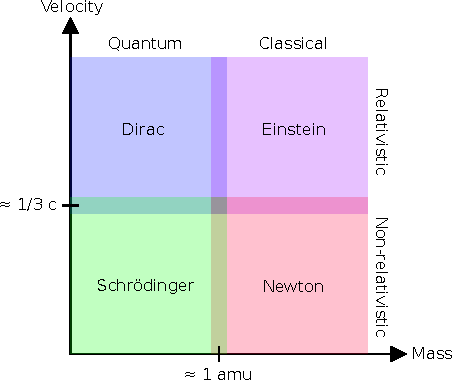
\includegraphics[scale=1.0]{Pics/dyneq}
\caption{Dynamical equations can be divided into four regimes, depending on the size and speed of the individual particles. Adapted form \cite{Jen2017}}
\label{fig:REGIMES}
\end{figure}

\section{The Electronic Schrödinger Equation}

\begin{quote}
  "Where did we get that [Schrödinger's equation] from? It's not possible to derive it from anything you know. It came out of the mind of Schrödinger."
  \begin{flushright}
    \small{--- \textit{Richard Feynman, The Feynman Lectures on Physics}}
  \end{flushright}
\end{quote}

If one is interested in describing the electron distribution in detail, the Schrödinger Equation (SEQ) is the best starting point. There is no formal, rigorous proof for the Schrödinger equation, similar to how Newton's second law cannot really be "derived", more than simply "motivated" by observation. 

As successful as the Schrödinger equation is, finding solutions to it is non-trivial. Different approximations may be applied to the SEQ to solve it more easily, without considerable loss of accuracy. 

\subsection{The Time-Independent Schrödinger Equation}

The potential energy operator is the only time-dependent part of the Hamiltonian:
\begin{equation}
\hat{H}(\mbf{r},t) = \hat{T}(\mbf{r}) + \hat{V}(\mbf{r},t)
\end{equation} 
\noindent For systems where the potential is time-independent, e.g. bound systems without external (electromagnetic) perturbation, the Hamiltonian is time-independent as well, which in turn allows to separate space and time variables. It can then be shown that the \emph{time-independent} Schrödinger equation takes the form
\begin{equation}
\hat{H}\Psi(\mbf{r}) = E \Psi(\mbf{r})
\end{equation}
\noindent where $E$ is the total energy of the system, and the eigenvalue of the wave function $\Psi$. The time-dependence is then simply reduced to a phase factor:
\begin{equation}
\Psi(\mbf{r},t) = e^{-iEt} \Psi(\mbf{r})
\end{equation}
\noindent 

\subsection{The Born-Oppenheimer Approximation}

Atomic nuclei are much heavier than electrons ($m_{proton} \approx 1836 m_{electron}$), and move much slower. To a good approximation, the nuclei can be assumed to be stationary from the point of view of electrons. This is known as the \emph{Born-Oppenheimer approximation}. The total Hamiltonian operator can be written in terms of the kinetic and potential operator of the nuclei ($n$) and electrons ($e$) as
\begin{equation}
\hat{H}_{tot} = \hat{T}_n + \hat{T}_e + \hat{V}_{ne} + \hat{V}_{ee} + \hat{V}_{nn}
\label{eq:FULLHAMILTONIAN}
\end{equation}
\noindent In the Born-Oppenheimer approximation, the kinetic energy of the nuclei $T_{nn}$ is neglected, and the nucleus-nucleus potential $V_{nn}$ is taken as a constant, which corresponds to neglecting the coupling between electrons and nuclei. This allows a separation of the electronic and nuclear variables. The remaining terms of Equation \ref{eq:FULLHAMILTONIAN} form the electronic Hamiltonian $\hat{H_{elec}}$. The solutions to the \emph{electronic Schrödinger equation}
\begin{equation}
\hat{H}_{elec} \Psi_{elec}(\mbf{r}_i, \mbf{R}_n ) = E_{elec}(\mbf{R}_n) \Psi_{elec}(\mbf{r}_i, \mbf{R}_n )
\end{equation}
\noindent produce the electronic wave function which depends on the (fixed) \emph{position} $\mbf{R}_n$ of the nuclei and no longer on the \emph{momentum} of the nuclei. The total energy
\begin{equation}
E_{tot}(\mbf{R}_n) = E_{elec}(\mbf{R}_n) + E_{nucl}(\mbf{R}_n)
\end{equation} 
\noindent provides a \emph{potential energy surface} (PES) on which the nuclei move. The PES can then be used to solve the nuclear Schrödinger equation to obtain information on vibrational, rotational and translational properties in the molecular system.

From this point onward, the subscript $elec$ is dropped, and only the electronic Schrödinger Equation is considered.

\section{Solutions to the Electronic Schrödinger Equation}

\subsection{Slater Determinants}

It is beneficial to first consider the wave function of the single electrons. In single-atom systems, these functions take the form of "atomic orbitals" (AOs). Correspondingly, "molecular orbitals" (MOs) are defined as the single electron wave functions in a molecular system. These spatial orbital functions form the basis of the total electronic wave function.  

The Hamiltonian in \ref{eq:FULLHAMILTONIAN} only depends on the spatial coordinates. However, to fully describe an electron, one also needs to consider spin. This is done by introducing two orthonormal spin functions $\alpha(\omega)$ and $\beta(\omega)$ corresponding to spin-up ($\uparrow$) and spin-down ($\downarrow$), with the spin-coordinate $\omega$. For one spatial molecular orbital, this gives two possible \emph{spin-orbitals}
\begin{equation}
\phi(\mathbf{x}) = \left\lbrace\begin{matrix}
\varphi(\mathbf{r}) \alpha(\omega) \\
\varphi(\mathbf{r}) \beta(\omega)
\end{matrix} \right.
\end{equation}
\noindent where $\varphi$ are the \emph{spatial orbitals}, and $\mathbf{x}$ are the combined spatial and spin coordinates. The spin orbitals therefore depend on four variables.

To a first approximation, one may consider a molecular system to consist of $N$ \emph{non-interacting}, independent electrons. The Hamiltonian is then written as a sum of one-particle Hamiltonians 
\begin{equation}
\mathbf{H} = \sum_i^N \mathbf{h}_i 
\end{equation}
\noindent Electron correlation may then be included in some average way by using \emph{effective} one-electron Hamiltonians, which is the basic working idea of the \emph{Hartree} method. The solution to the SEQ can then be expressed as a product of the one electron wave functions
\begin{equation}
\Psi^{HP}(\mbf{x}_1,\mbf{x}_2,...,\mbf{x}_N) = \phi(\mbf{x}_1) \phi(\mbf{x}_2) ... \phi(\mbf{x}_N)
\end{equation}
\noindent which is also known as \emph{Hartree product}. 

However, the Hartree product does not take into account the \emph{indistinguishability} of electrons. In what is known as the antisymmetry principle, a generalization of the Pauli exclusion principle, the wave function needs to fulfill 
\begin{equation}
\Psi(\mbf{x}_1,\mbf{x}_2) = - \Psi(\mbf{x}_2,\mbf{x}_1) 
\end{equation}
\noindent upon exchange of any two electrons in the system. This is most easily achieved by using \emph{Slater determinants} (SD). For a molecular system consisting of $N$ electrons distributed over $N$ spin orbitals $\phi_i$, the SD takes the form
\begin{equation}
\Psi_{SD}(\mbfx_1, \mbfx_2, \ldots, \mbfx_N) = \frac{1}{\sqrt{N!}}
\begin{vmatrix}
\phi_I(\mbfx_1) & \phi_J(\mbfx_1) & \ldots & \phi_P(\mbfx_1) \\
\phi_I(\mbfx_2) & \phi_J(\mbfx_2) & \ldots & \phi_P(\mbfx_2) \\
\vdots & \vdots & \ddots & \vdots \\
\phi_I(\mbfx_N) & \phi_J(\mbfx_N) & \ldots & \phi_P(\mbfx_N) \\
\end{vmatrix}
\end{equation}
\noindent Or, using the diagonal of the SD as a short-hand notation
\begin{equation}
\Psi_{SD}(\mbfx_1, \mbfx_2, \ldots, \mbfx_N) = \ket{\phi_I(\mbfx_1) , \phi_J(\mbfx_1), \ldots, \phi_K(\mbfx_1)}
\end{equation}

\subsection{The Fock Space}

A more generalized representation of the space of the antisymmetrized electron wave functions can be achieved by introducing the concept of occupation number (ON) vectors in the context of second quantization (Annex). In a system with $M$ possible states (in this case spin molecular orbitals), the ON vectors take the form
\begin{equation}
\ket{\mbf{k}} = \ket{k_1, k_2, \ldots, k_M} = 
\left\lbrace
\begin{matrix}
1 \quad \textit{if $\phi_P$ occupied} \\
0   \quad \textit{if $\phi_P$ occupied}
\end{matrix}
\right.
\label{eq:ONVECTORS}
\end{equation}
\noindent The occupation number is 1 if $\phi_P$ is present in the SD, and 0 if not. Together, all possible ON vectors in Equation \ref{eq:ONVECTORS} form an orthonormal abstract vector space, known as Fock space. The Fock space formed by $N$ electrons distributed over $M$ orbitals is denoted as $F(M,N)$ with total dimension equal to the binomial coefficient $\smash{{M\choose N}}$. The sum of the occupation numbers in the ON vectors gives the total number of electrons
\begin{equation}
N = \sum_i^M k_i
\end{equation}
\noindent The special Fock space $F(0,M)$ contains a single vector known as the vacuum state with
\begin{align}
\ket{vac} &= \ket{0_1, 0_2, \ldots, 0_M} \\
\bra{vac}\ket{vac} &= 1
\end{align}
\noindent The ON vectors in $F(M,N)$ can be alternatively expressed in terms of the vacuum state from $F(M,0)$ using creation operators
\begin{equation}
\ket{\mbf{k}} = \left[ \prod_{P=1}^M (a\pdg_P)^{k_P} \right] \ket{vac}
\end{equation}
\noindent In second quantization, the antisymmetry principle of the wave function is guaranteed by the commutator relationship of the annihilation and creation operators $a_P$ and $a\pdg_P$ which act on the ON vectors.

\subsection{Exact Solution and Standard Models}

The simplest approach to solving the electronic SEQ is by approximating the exact wave function $\Psi$ using a single Slater determinant where the electrons occupy the lowest lying molecular orbitals. The Hartree-Fock method is an example of a \emph{single-determinant method} and finds \emph{the} single best Slater determinant for $\ket{\Psi}$. In Fock space, the best possible determinant is represented by the ON vector where the $N$ lowest lying orbitals are occupied. 

As will be discussed in more detail later, a single-determinant treatment of the electronic wave function is insufficient to fully capture \emph{electron correlation}. The electron correlation energy is formerly defined as the difference between the Hartree-Fock energy and the \emph{exact} energy of $\ket{Psi}$
\begin{equation}
E_{correlation} = E_{HF} - E_{exact}
\end{equation}
\noindent although the Hartree-Fock wave function does include correlation effects to some degree. In a more general sense, electron correlation is a broad term for any interactions between electrons that make their movement depend on each other, or \emph{correlate} with each other (see Section \ref{sec:CORRELATION}). 

In order to improve on the HF approximation, it is important to add additional Slater determinants. These SDs can be generated from the HF reference wave function by replacing the occupied MOs $\phi_I$ in a reference Slater determinant by one or multiple orbitals $\phi_A$ which were previously unoccupied. This effectively corresponds to exciting one or more electrons from their occupied molecular orbitals $I,J,..$ to unoccupied, or $virtual$ orbitals $A,B,..$. These excited Slater determinants can be classified by the number of electrons they excite and are often referred to as singles, doubles, triples and so on.
\begin{align}
\ket{\Phi_0} &= \ket{HF} \\
\ket{\Phi_{I}^{A}} &= a\pdg_A a_I \ket{HF} \\
\ket{\Phi_{IJ}^{AB}} &= a\pdg_A a_I a\pdg_B a_J \ket{HF} \\
\ket{\Phi_{IJK}^{ABC}} &= a\pdg_A a_I a\pdg_B a_J a\pdg_C a_K \ket{HF} \\
\ldots & 
\end{align}
\noindent Alternatively, singles states are known as 1-particle-1-hole (1p-1h or simply p-h) states, doubles as 2-particle-2-hole (2p-2h) and so on, due to the excitation operators effectively creating \emph{holes} in the reference determinant and adding \emph{particles} in higher lying orbitals instead. 

The exact solution to the electronic Schrödinger equation is then given by the sum of the Hartree-Fock wave function and all possible ON vectors in $F(M,N)$
\begin{equation}
\ket{\Psi} = c_0 \ket{HF} + \sum^{{{M}\choose{N}}-1}_{i=1} c_i  \ket{i} 
\label{eq:EXACTWF}
\end{equation}  
\noindent Equation \ref{eq:EXACTWF} offers a systematic approach to improve on the Hartree Fock method, by increasing (1) the number of Slater determinants and (2) the basis set size $M$, and gives rise to a hierarchy of methods (Figure \ref{fig:STANDARDMODEL}). Correlated electronic structure methods mainly differ by how they determine the expansion coefficients $c$. For all but the smallest systems, the full $F(M,N)$ Fock space cannot be used in calculations due to the total number of ON vectors which increases binomially with $\smash{{M}\choose{N}}$, and hence the number of coefficients to be determined. In practice, the Fock space is \emph{truncated} to some degree.

\begin{figure}
\centering
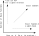
\includegraphics[scale=2.0]{Pics/standardmodel}
\caption{The wave function converges to the exact solution in the limit of an infinitely large basis set that spans the molecular orbitals, and an infinitely large correlation space spanned by the Slater Determinants.}
\label{fig:STANDARDMODEL}
\end{figure}

\emph{Multi-determinant} methods like configuration interaction (CI) or coupled cluster (CC) use the Hartree Fock wave function as the reference from which they generate singles, doubles, triples ... SDs. By truncating at different excitation levels, one gets a hierarchy of CI/CC methods which recover different amounts of correlation energy (e.g. CIS, CISD, CISDT ...). Multi-determinant methods are mainly suited to recover dynamic correlation.

For systems with strong static correlation, additionally, a multi-reference approach is needed. Here, the excited SDs are generated from multiple reference states rather than only from HF. Methods include multi-reference CI (MRCI) and multi-reference CC (MRCC). The reference states are traditionally obtained from multi-configurational self-consistent-field methods (MCSCF) like the complete active space SCF (CASSCF) or restricted active space SCF (RASSCF). MCSCF is a combination of HF and CI, which both optimizes the HF molecular coefficients and the CI expansion coefficients. Multi-reference methods methods mainly recover \emph{static correlation}. 

\subsection{The Variational Method}

The time-independent Schrödinger equation takes the form of an eigenvalue problem
\begin{equation}
\hat{H} \ket{\Psi_i} = E_i \ket{\Psi_i} \qquad i=0,1,2,...\infty
\label{eq:SEQINFTY}
\end{equation}
\noindent where the infinite set of exact solutions $\ket{\Psi_i}$ with eigenvalues $E_i$ forms an orthonormal basis
\begin{equation}
\bra{\Psi_i}\ket{\Psi_j} = \delta_{ij}
\end{equation} 
\noindent A trial wave function can be expanded in the basis of exact solutions with coefficients $c$ as
\begin{equation}
\ket{\tPsi} = \sum_i a_i \ket{\Psi_i}
\label{eq:trialwave}
\end{equation}
\noindent The \emph{variation principle} states that the expectation value of the Hamiltonian of an approximate wave function of the form \ref{eq:trialwave} is an upper bound to the exact ground state energy. This statement can be expressed as
\begin{equation}
\frac{\bra{\tPsi}\hat{H}\ket{\tPsi}}{\vphantom{\widetilde{\Psi}} \bra{\tPsi}\ket{\tPsi}} \geq E_0
\end{equation}
\noindent The equality only holds when $\ket{\tPsi}$ is equal to the exact solution $\ket{\Psi_0}$. One can recast the eigenvalue problem \ref{eq:SEQINFTY} as a variational optimization problem where the energy is a functional of a trial wave function
\begin{equation}
E[\tPsi] = \frac{\bra{\tPsi}\hat{H}\ket{\tPsi}}{\vphantom{\widetilde{\Psi}} \bra{\tPsi}\ket{\tPsi}}
\end{equation}
\noindent The saddle points of the energy functional then correspond to the exact solutions of the Schrödinger equation. The variational approach to the SEQ provides a powerful tool to solve a wide variety of problems in electronic structure theory.

The trial wave function depends on a set of coefficients $c$, and hence the energy functional will also depend on these coefficients. In general, determining the coefficients which minimize the functional is very difficult. However, a more simple approach of the variational method can be obtained by using a linear ansatz where the trial function is expanded in a fixed N-dimensional set of orthonormal basis functions $\ket{\phi}$
\begin{equation}
\ket{\tPsi} = \sum^N_i c_i \ket{\phi_i}
\end{equation}
By using Lagrange's method of undetermined multipliers
\begin{align}
\mathcal{L}(\mbf{c},E) &= \bra{\tPsi}\hat{H}\ket{\tPsi} - E(\bra{\tPsi}\ket{\tPsi} - 1) \\
\frac{\partial \mathcal{L}}{\partial \mathcal{\mbf{c}}} &= 0
\end{align}
\noindent it is possible to show that the variational problem corresponds to solving the eigenvalue problem involving the Hamiltonian matrix $\mbf{H}$:
\begin{equation}
\mbf{H}\mbf{c}_n = E_n \mbf{c_n}
\end{equation}
\noindent Or, in a more general form
\begin{equation}
\mbf{H}\mbf{C} = \mbf{C}\mbf{E}
\end{equation}
\noindent Here, $\mbf{C}$ is a $N$ by $N$ coefficient matrix containing $N$ column coefficient vectors $\mbf{c}_n$ ($n$ = $0...N$) which describe $N$ possible solutions for the trial wave function $\ket{\tPsi}$. $\mbf{E}$ is a diagonal matrix containing the eigenvalues $E_n$. This approach of finding approximate solutions to the eigenvalue problem \ref{eq:SEQINFTY} is known as the \emph{linear variational method}. 

\section{Hartree-Fock}

The Hartree-Fock method is central to electronic structure method. It is computationally inexpensive, and is still routinely used in qualitative studies of large molecules, even if it does not accurately account for electron correlation. It also serves as the starting point for correlated methods. Only a few computational methods actually bypass the solution to the Hartree-Fock equations, firmly cementing its place in quantum chemistry.

\subsection{The Hartree Fock Equations}

Recall the structure of the electronic Hamiltonian
\begin{equation}
\hat{H} = \hat{T}_e + \hat{V}_{ne} + \hat{V}_{ee} + \hat{V}_{nn}
\end{equation}
\noindent with
\begin{align}
\hat{T}_e &= -\sum_i^N \frac{1}{2} \nabla_i^2 \qquad \textrm{kinetic energy of electrons} \\
\hat{V}_{ne} &= -\sum_a^{N_{nuc}} \sum_i^N \frac{Z_a}{\mid\mbf{R}_a - \mbf{r}_i\mid} \qquad \textrm{nuclei-electron repulsion} \\
\hat{V}_{ee} &= \frac{1}{2} \sum^N_i \sum^N_{j \neq i} \frac{1}{\mid \mbf{r}_i - \mbf{r}_j\mid} \qquad \textrm{electron-electron repulsion} \\
\hat{V}_{nn} &= \frac{1}{2}\sum_a^{N_{nuc}} \sum_{b \neq a}^{N_{nuc}} \frac{Z_a Z_b}{\mid \mbf{R}_a - \mbf{R}_b \mid} \qquad \textrm{nuclei-nuclei repulsion} 
\end{align}
\noindent In Hartree-Fock theory, the electrons are treated as independent particles. One can therefore ignore the coupling between electrons in $\hat{V}_{ee}$ and express the Hamiltonian as a sum of an effective one-electron operator $\mbf{f}$, also known as the \emph{Fock} operator, of the form
\begin{align}
\hat{H} &= \sum_i \hat{f}_i =  \sum_i \mbf{h}_i + \frac{1}{2} \sum_i \sum_{j \neq i} \mbf{g}_ij  \\
\hat{h}_i &= -\frac{1}{2}\nabla_i^2 - \sum_a^{N_{nuc}} \frac{Z_a}{\mid \mbf{R}_a - \mbf{r}_i |} \\
\hat{g}_{ij} &= \frac{1}{\mid \mbf{r}_i - \mbf{r}_j \mid}
\end{align}
\noindent The one-electron operator $\hat{h}$, also known as the \emph{core} Hamiltonian describes the movement of the electrons in the field of the nuclei. The two-electron operator $\mbf{g}_{ij}$ gives the average potential (or "field") experienced by electron $i$ due to the presence of all the other electrons $j$. For this reason, Hartree-Fock is also known the \emph{mean-field} approximation. In second quantization, the Fock operator takes the form
\begin{equation}
\hat{f} = \sum^{M}_{PQ} h_{PQ} a\pdg_P a_Q + \frac{1}{2} \sum^{M}_{PQRS} g_{PQRS} a\pdg_P a\pdg_R a_S a_Q
\label{eq:FOCK2Q}
\end{equation}
\noindent with the matrix elements of the one and two electron operators given by
\begin{align}
h_{PQ} &= \bra{\phi_P} \mbf{h} \ket{\phi_Q} = \int \phi_P^*(\mbf{x}) h(\mbf{x}) \phi_Q(\mbf{x}) d\mbf{x} \\
g_{PQRS} &= \bra{PQ}\ket{RS} = \int\int \phi_P^*(\mbf{x}_1) \phi^*_R(\mbf{x}_2) g(\mbf{x}_1,\mbf{x}_2) \phi_Q(\mbf{x}_1) \phi_S(\mbf{x}_2) d\mbf{x}_1 d\mbf{x}_2
\end{align} 
\noindent The elements $g_{PQRS}$ are known as the 2-electron repulsion integrals. Calculating the expectation values for the Fock operator in \ref{eq:FOCK2Q} using second quantization gives:
\begin{equation}
\begin{split}
f_{PQ} &= \bra{\phi_P} \mbf{f} \ket{\phi_Q} \\
	&= h_{PQ} + \sum_{I}^N \frac{1}{2} (g_{PQII} - g_{PIIQ}) \\
	&= h_{PQ} + \frac{1}{2} (J_{PQ} - K_{PQ})
\end{split}
\end{equation} 
\noindent The symmetric matrix with entries $f_{PQ}$ is also known as the \emph{Fock matrix}. $\mbf{J}$ is the \emph{coulomb matrix} and describes electron correlation due to the coulomb potential (coulomb correlation), and $\mbf{K}$ is the exchange matrix describing the electron correlation which arises due to the Pauli exclusion principle (Fermi correlation). The exchange contributions have no classical counterpart and arise purely from quantum mechanical considerations. 

In the special basis where the Fock matrix is diagonal
\begin{equation}
f_{PQ} = \delta_{PQ} \eps_P 
\end{equation}
\noindent the one-electron eigenfunctions of the Fock operator 
\begin{equation}
\mbf{f} \ket{\phi_P} = \eps_P \ket{\phi_P} 
\label{eq:HFEQ}
\end{equation} 
\noindent are known as the \emph{canonical molecular spin orbitals}, and the eigenvalues are the \emph{molecular orbital energies}. Solving the \emph{canonical Hartree-Fock equation} \ref{eq:HFEQ} gives the MOs which form the basis of the Hartree-Fock wave function. It should be stressed that the total electronic Hartree-Fock energy is not the sum of the individual MO energies, but is given by the expectation value of the Hamiltonian 
\begin{equation}
E_{HF} = \bra{HF}\mbf{H}\ket{HF} = \sum_{I}^{N} h_{II} + \frac{1}{2} \sum_{I}^{N} \left( J_{II} - K_{II} \right)   
\end{equation}
\noindent where the sum runs over the \emph{occupied} orbitals $I$. For $N$ electrons distributed over $M$ MOs, there are $N$ occupied orbitals with $\eps_I < 0$ and $M-N$ virtual orbitals with $\eps_A > 0$. 

\subsection{The Basis Set Approximation}

Up until this point, the electronic wave function was constructed from Slater determinants of molecular spin orbitals. Virtually all applications use a basis set expansion to express the unknown MOs in terms of known functions, conventionally called \emph{atomic orbitals}. Any type of function can be used, e.g. exponentials, Gaussians, polynomials or plane waves. The molecular orbitals are then expressed as a \emph{linear combination of atomic orbitals} (LCAO)
\begin{equation}
\ket{\phi_i} = \sum_i^{M_{basis}} c_{i\mu} \chi_{\mu} 
\end{equation}
\noindent For molecular systems, there are two types of basis functions that are generally used, namely Slater Type Orbitals (STO) and Gaussian Type Orbitals (GTO):

\begin{align}
\chi_{\zeta, n, l, m}^{STO} (r,\theta ,\phi ) = N Y_{l,m} (\theta , \phi ) r^{n-1} e^{-\zeta r}
\\
\chi_{\zeta, n, l, m}^{GTO} (r,\theta ,\phi ) = N Y_{l,m} (\theta , \phi ) r^{2n - 2 - l} e^{-\zeta r^2}
\end{align}

\noindent where N is a normalization constant and $Y_{l,m}$ are spherical harmonics. There are two major differences between STOs and GTOs. At r = 0, STOs have finite slope and GTOs have zero slope. For large r values, GTOs decay much more rapidly than STOs. From an electronic structure point of view, one would prefer to use STO, as they describe the qualitative features of molecular orbitals better than GTOs. Roughly three time as many GTOs are necessary to obtain the same accuracy as with STOs. Nonetheless, GTOs are preferred, as their drawbacks are outweighed by the relative ease with which integrals of GTOs can be evaluated compared to STOs.

\subsection{Working Equations for Restricted and Unrestricted Hartree-Fock}

For reasons of efficient implementation, it is useful to separate out different electron spin components. The Fock matrix has four spin blocks: $F_{\alpha\alpha}$, $F_{\alpha\beta}$, $F_{\beta\alpha}$ and $F_{\beta\beta}$. The Fock matrix in the canonical basis is diagonal, and therefore only the diagonal blocks  $F_{\alpha\alpha}$ and $F_{\beta\beta}$ are important. Introducing the notation $\olI$ for MOs with spin $\sigma'$, and $I$ with opposite spin $\sigma$, the matrix elements of a spin block are given by
\begin{equation}
\begin{split}
f_{PQ}^{\sigma} &= h_{PQ}^{\sigma} + \frac{1}{2} \left\lbrace \sum^{N_{\sigma}}_{PQ}\sum^{N_{\sigma}}_{I} \cn{PQ}{II} - \cn{PI}{QI}  - \sum^{N_{\sigma}}_{PQ}\sum^{N_{\sigma'}}_{I} \cn{PQ}{\olJ\olJ} - \cn{P\olJ}{Q\olJ} \right\rbrace \\
&= h_{PQ}^{\sigma} + \sum^{N_{\sigma}}_{PQ} J^{\sigma}_{PQ} - K^{\sigma}_{PQ} + J^{\sigma'}_{PQ} - K^{\sigma'}_{PQ}
\end{split}
\end{equation}
\noindent The opposite spin block $f_{PQ}^{\sigma'}$ is obtained by substituting indices with a bar by indices without a bar and vice-versa. Spin separation yields two coupled sets of equations for alpha and beta MOs
\begin{equation}
\begin{split}
\mbf{f}^{\alpha} \ket{\phi^{\alpha}_I} &= \eps^{\alpha}_I \ket{\phi^{\alpha}_I} \\
\mbf{f}^{\beta} \ket{\phi^{\beta}_I} &= \eps^{\beta}_I \ket{\phi^{\beta}_I} 
\end{split}
\label{eq:UHF}
\end{equation} 
\noindent These are known as the unrestricted Hartree-Fock equations (UHF). For closed-shell molecules with equal number of alpha and beta electrons, the spatial part of the MOs is the same for both spins. The expression for the Fock matrix then further simplifies to 
\begin{equation}
f_{ij} = h_{ij} + 2J_{ij} - K_{ij} 
\end{equation}
\begin{equation}
\mbf{f} \ket{\phi_i} = \eps_i \ket{\phi_i}
\label{eq:RHF}
\end{equation}
\noindent The equations in \ref{eq:RHF} are known as the restricted Hartree-Fock (RHF) equations. 

\noindent Using the linear variatonal method explained in the previous section for the MO trial functions expressed as a linear combination of $N_{bas}$ AO basis functions, the eigenvalue problem for RHF can be recast in matrix form as
\begin{align}
\mbf{F} \mbf{C} &= \mbf{C} \mbf{E} 
\end{align}
\noindent with the MO coefficient matrix $\mbf{C}$ and the Fock matrix $\mbf{F}$ in the AO basis given by
\begin{align}
F_{\mu\nu} &= H^{core}_{\mu\nu} + \sum_{\lambda\sigma}^{N_{basis}} \left(2 \cn{\mu\nu}{\sigma\lambda} P_{\lambda\sigma} - \cn{\mu\sigma}{\nu\lambda} P_{\lambda\sigma} \right) \\
&= H^{core}_{\mu\nu} + 2 J_{\mu\nu} - K_{\mu\nu} 
\end{align}
\noindent The symmetric matrix $\mbf{P}$ is the so-called atomic orbital density matrix (DM) of the form
\begin{equation}
P_{\mu\nu} = \sum_i^{N_{occ}} C_{\mu i} C_{\nu i} 
\end{equation}
\noindent A similar expressions is found for UHF
\begin{equation}
\begin{split}
F_{\mu\nu}^{\sigma} &= H^{core}_{\mu\nu} + \sum_{\lambda\sigma}^{N_{basis}} \left( \cn{\mu\nu}{\sigma\lambda} P^{T}_{\lambda\sigma} - \cn{\mu\sigma}{\nu\lambda} P^{\sigma}_{\lambda\sigma} \right) \\
P^T_{\mu\nu} &= P^{\sigma}_{\mu\nu} + P^{\sigma'}_{\mu\nu} 
\end{split}
\end{equation}
\noindent where the AO spin-density matrices $\mbf{P}^{\sigma}$ are defined as the product of the corresponding coefficient matrices with spin $\sigma$.  

\subsection{The Self-Consistent Field Method}

In general, the atomic orbitals are not orthogonal. The overlap matrix $\mbf{S}$ is defined as 
\begin{equation}
S_{\mu\nu} = \int \chi_{\mu}^*(\mbf{r}) \chi_{\nu}^*(\mbf{r}) d\mbf{r}
\end{equation}
\noindent with diagonal entries $S_{\mu\mu} = 1$, and off-diagonal elements $0 < \mid S_{\mu\nu} \mid < 1$. The eigenvalue problem for RHF then takes the more general form
\begin{equation}
\mbf{F} \mbf{C} = \mbf{SC} \mbf{E}
\label{eq:RHALL}
\end{equation}
\noindent The equations in \ref{eq:RHALL} are known as the \emph{Roothan-Hall equations}. In the unrestricted case, they are called the \emph{Pople-Nesbet equations} which are given by
\begin{align}
\mbf{F}^{\alpha} \mbf{C}^{\alpha} &= \mbf{SC}^{\alpha} \mbf{E}^{\alpha} \\
\mbf{F}^{\beta} \mbf{C}^{\beta} &= \mbf{SC}^{\beta} \mbf{E}^{\beta}
\end{align}  
\noindent The Fock matrix is constructed using the coefficient matrices $\mbf{C}$ to compute the density matrix $\mbf{P}$. This means that the RH (and PN) equations depend on their own solution and must be solved iteratively. Popular choices for iterative schemes include \emph{Newton's} method and the \emph{self-consistent field} (SCF) method, with the latter being the most straight-forward one to implement. 

The SCF procedure is summarized in Algorithm \ref{algo:SCF}. At every iteration, the Fock matrix is diagonalized to obtain a new guess for the density matrix, which is used for constructing the Fock matrix in the next step. These steps are repeated until \emph{self-consistency} is reached. There are different ways to test for convergence, the simplest being the Hartree-Fock energy difference between subsequent iterations. A more rigorous bound is given by the matrix norm of the error vector $\mbf{e}$
\begin{equation}
\mbf{e} = \mbf{FPS} - \mbf{SPF} 
\end{equation}
\noindent At convergence, the density matrix commutes with the Fock matrix though the overlap matrix. 

\begin{algorithm}
\KwIn{Molecule with nuclear coordinates $\{\mbf{R}_A\}$, atomic numbers $\{Z_A\}$, number of electrons $N$ and basis set $\{\chi_{\mu}\}$}
\KwOut{The matrices $\mbf{F}$, $\mbf{P}$, $\mbf{C}$ and $\mbf{E}$} 
Calculate all one- and two electron integrals
\\
Compute the transformation matrix $\mbf{X}$ from the overlap matrix $\mbf{S}$ with
\begin{equation}
\mbf{X}\pdg \mbf{SX} = \mbf{1} 
\end{equation}
\\
Generate a set of guess orbitals to compute an initial guess density $\mbf{P}$
\\
\While{not converged}{
	Construct the Fock matrix $\mbf{F}$ using the current guess density
	\\
	Orthogonalize the Fock matrix $\mbf{F'} = \mbf{X}\pdg \mbf{FX}$
	\\
	Diagonalize $\mbf{F}'$ to obtain the new orthogonalized MO coefficient matrices $\mbf{C}'$
	\\
	Compute $\mbf{C} = \mbf{X}\mbf{C}$
	\\
	Form the new density $\mbf{P} = \mbf{CC}^T$
	\\
	Check convergence using certain criteria
}
\caption{Hartree-Fock Self-Consistent Field}
\label{algo:SCF}
\end{algorithm}

\subsubsection{SCF Initial Guesses}

The preiteration steps compute the two-electron integrals, the transformation matrix $\mbf{X}$ and a set of guess orbitals. There are different methods for generating a guess. The closer the guess is to the solution, the fewer SCF iterations are needed which saves time. The simplest method consists in using a null matrix for $\mbf{P}$, which corresponds to setting the Fock matrix to the core Hamiltonian $\mbf{H}^{core}$. Diagonalization then gives the guess orbitals. The core Hamiltonian gives a sufficiently close starting guess for small molecules, but is unsuitable for larger molecules. 

The most popular and efficient method at the time of writing is the superposition of atomic densities (SAD) (ref). For each type of atom in the molecule, an atomic HF calculation is carried out which gives the atomic density matrix for this atom type. The molecular guess density matrix is then constructed by setting its diagonal blocks to to the atomic densities. The SAD method generates densities that are quite close to the solution. For implementation details, see Annex \ref{app:SCFGUESS}.

An alternative starting guess can be obtained by first carrying out a HF calculation with a smaller basis set using the core or SAD guess, and then projecting the density matrix onto the larger basis set (Annex \ref{app:SCFGUESS}). This method is especially useful for larger basis sets.  

\subsubsection{SCF convergence}

There is no guarantee that the SCF procedure converges. For small molecules and equilibrium geometries, the unmodified SCF procedure converges quite smoothly. For large, diffuse basis sets or distorted geometries, additional modifications to the algorithms might be necessary:
\begin{enumerate}
\item Direct inversion of the iterative subspace (DIIS): the previous Fock matrices are used for extrapolation to generate a better Fock matrix (Annex \ref{sec:DIIS})
\item Damping: A damping factor $\omega$ is introduced and the density matrix is replaced by a weighted average $\mbf{P}'_{n+1} = \omega \mbf{D}_n + (1-\omega)\mbf{D}_{n+1}$. Damping is especially useful when the SCF energy oscillates around the equilibrium
\item Level shifting: It has been shown that raising the energy of the virtual orbitals guarantees convergence, at the cost of a decreased convergence rate
\end{enumerate} 

\subsection{Brillouin's Theorem and Orbital Rotations}

The Fock matrix can be divided into four distinct blocks: occupied-occupied, occupied-virtual, virtual-occupied and virtual-virtual. The terms "particle" (p) and "hole" (h) may be used instead of occupied and virtual. In the special case where the orbitals are the canonical MOs, the Fock matrix is diagonal. This is known as the \emph{canonical condition} for the HF wave function. However, diagonality is not necessary for obtaining a valid HF wave function. The general Hartree-Fock equations take the form
\begin{equation}
\hat{f} \phi_P = \sum_{PR} \lambda_{PR} \phi_R
\end{equation}
\noindent Where $\lambda$ are the Lagrange multipliers. For non-canonical MOs, the p-p and h-h are non-diagonal, with elements $\lambda_{IJ}$ and $\lambda_{AB}$ respectively. The off-diagonal elements are computed as
\begin{equation}
f_{IA} = \sbra{HF}\hat{f}\sket{a\pdg_A a_I HF} = 0
\end{equation}
\noindent and are zero by virtue of \emph{Brillouin's theorem}. This is also known as the \emph{variational condition} for the HF wave function; it is an alternative formulation of the variational principle (see \cite{Hel2000}, section 10.3.5).

The Hartree-Fock energy is therefore stable under unitary rotations
\begin{equation}
\phi_{I'} = \mbf{U} \phi_I \qquad U\pdg U = \mbf{U}
\end{equation}
\noindent The canonical MOs may be rotated to give another orbital representation with smaller spatial extent, also known as localized molecular orbitals (see Section \ref{sec:ABCLMO}).

\section{Electron Correlation \label{sec:CORRELATION}}

In the Hartree-Fock method, the electron-electron interaction is replaced by an average interaction. For large basis sets, H is actually able to recover approximately 99\% of the electron correlation. Unfortunately, the remaining 1\% are often important to compute chemical properties with sufficient accuracy.

Electron correlation arises from electrons trying to avoid each other due to coulombic repulsion (coulomb correlation) and the antisymmetry principle (Fermi correlation). This in turn leads to a region of space around each electron where the probability of finding another electron is reduced, typically known as the \emph{coulomb hole} for electrons of opposite spin, and \emph{Fermi hole} for electrons of the same spin. 

Another distinction is often drawn between \emph{dynamic correlation} and \emph{static correlation}, although there exists no formal definition. Dynamic correlation generally describes the correlated movement of electrons due to their "instantaneous mutual repulsion" \cite{Jen2017}. For example, in the ground-state Helium atom, electron correlation is purely dynamical. Static (or non-dynamic) correlation on the other hand arises in the case of near-degeneracy, where multiple configurations of similar energy contribute to the ground-state wave function. To show the difference between these two two types of correlation, the dissociation of the H$_2$ molecule is often taken as an illustrative example. At equilibrium distance, correlation is mostly dynamic, and the ground-state can be well described as a singlet state. In the dissociation limit, electrons may be coupled to yield either a singlet \emph{or} a triplet, as the energy difference between those two states vanishes (Figure?). The correlation in the system in then entirely static. There is no clear-cut line between dynamic and static correlation, but it offers a useful classification for correlation effects.

To fully capture both dynamic and static correlation, it is crucial to add additional Slater determinants as mentioned previously. Methods which generate excited Slater determinants from a single reference SD recover mostly dynamical correlation: electrons are disturbed through their instantaneous repulsion and are excited to higher spin orbitals, hence the need of additional excited-type SDs. Methods generating SDs from multiple references recover mostly static correlation. At the theoretical limit (i.e. the full configuration space), both approaches eventually recover all correlation effects. It is therefore the responsibility of the computational chemist to choose the correct method that best fits the problem at hand.

Any electronic structure method that improves on the HF wave function is usually referred to as a "correlated method". Hartree-Fock, by convention, is an "uncorrelated method". 

For the rest of this report, only single-reference methods are considered.

\section{Configuration Interaction}

\subsection{The CI Matrix}

Configuration interaction (CI) is the simplest and one of the oldest examples of a correlated electronic structure method. The CI wave function takes the general form
\begin{equation}
\ket{CI} = \ket{\Psi_0} + \sum_{IA} c_{I}^{A} \ket{\Phi_{IA}} + \sum_{\substack{I < J \\ A < B}} c_{IJ}^{AB} \ket{\Phi_{IJ}^{AB}} + \sum_{\substack{I < J < K \\ A < B < C}} c_{IJK}^{ABC} \Phi_{IJK}^{ABC} + \dots
\end{equation}
\noindent summing all SDs of all possible types (singles, doubles, triples...). $\Phi_0$ is the reference wave function, here taken as the HF ground state. Whereas the HF wave function was a linear combination of molecular orbitals, the CI wave function is a linear expansion of SDs. Similarly, the CI expansion coefficient matrix $\mbf{C}$ are determined variationally
\begin{equation}
\frac{\partial}{\partial C_i} \frac{\bra{CI}\hat{H}\ket{CI}}{\bra{CI}\ket{C}}
\end{equation}
\noindent which, as was shown before, reduces to the eigenvalue problem
\begin{equation}
\mbf{H}\mbf{C} = \mbf{C}\mbf{E}
\end{equation}
\noindent The matrix $\mbf{H}$ is also known as the \emph{CI matrix}. Using the notation $\ket{S}$, $\ket{D}$, $\ket{T}$, ... to denote the set of singles, doubles, triples ... SDs, the CI matrix takes the form
\begin{equation}
\begin{bmatrix}
\bra{\Phi_0}\mbf{H}\ket{\Phi_0} & 0 & \bra{\Phi_0}\mbf{H}\ket{D} & 0 & 0 & \ldots \\
0 & \bra{S}\mbf{H}\ket{S} & \bra{S}\mbf{H}\ket{D} & \bra{S}\mbf{H}\ket{T} & 0 & \ldots \\
\bra{D}\mbf{H}\ket{\Phi_0} & \bra{D}\mbf{H}\ket{S} & \bra{D}\mbf{H}\ket{D} & \bra{D}\mbf{H}\ket{T} & \bra{D}\mbf{H}\ket{Q} & \ldots \\
0 & \bra{T}\mbf{H}\ket{S} & \bra{T}\mbf{H}\ket{D} & \bra{T}\mbf{H}\ket{T} & \bra{T}\mbf{H}\ket{Q} & \ldots \\
0 & 0 & \bra{D}\mbf{H}\ket{Q} & \bra{T}\mbf{H}\ket{Q} & \bra{Q}\mbf{H}\ket{Q} & \ldots \\
\vdots & \vdots & \vdots & \vdots & \vdots & \ddots  
\end{bmatrix}
\end{equation}
\noindent In analogy to the Fock matrix, some blocks in the CI matrix are zero. Brillouin's theorem states that there is no coupling between the ground state and the singlet states. That does not imply that they do not contribute to the CI energy at all. Singles mix \emph{indirectly} via doubles. Moreover, matrix blocks of the Hamiltonian between two SDs which differ by more than two spin orbital orbitals are also zero. Triples mix with doubles and singles, but not with the ground state.

A more compact representation of the CI matrix is obtained by taking linear combinations of SDs in the same excitation manifold, known as configuration state functions (CSF) or spin-adapted configurations (SAC). The CSFs form a basis smaller than that composed of all individual SDs which leads to computational savings. However, CSFs were primarly introduced to preserve the spin symmetry of the ground state, or in other words, CSFs are eigenfunctions of the $\mbf{S}^2$ operator. If the HF ground state is a singlet, a non-spin-symmetric CI basis may lead to the CI wave function being a mixture of singlet and triplet determinants. 

\subsection{Truncated CI}

Full CI, i.e. including all excitation manifolds, is only computationally feasible for all but the smallest molecules, due to the binomial increase in the number of SDs as a function of system and basis set size. For this reason, the CI wave function my be truncated at a given excitation level. Including only singles gives configuration interaction with singles (CIS), including singles and doubles yields configuration interaction with singles and doubles (CISD), etc. Higher order methods recover a larger fraction of the correlation energy, but come at a higher computational cost.

It should be noted that the energy of the CIS wave function is equal to the HF energy due to Brillouin's theorem, and hence does not contribute to the correlation energy of the ground state.  

\subsection{Solving the CI Eigenvalue Problem}

Even at relatively low truncation levels, the number of matrix elements have a quite steep polynomial scaling with $\ccpx{6}$ for CISD and $\ccpx{8}$ for CISDT. In most cases however, only the few lowest eigenvalues are needed. Davidson's method of matrix diagonalization (Annex \ref{ann:DAV}) was specifically developed to tackle this problem. Rather than storing the whole matrix, only matrix-vector products need to be computed
\begin{equation}
\mbf{r} = \mbf{M}_{CI} \mbf{u}
\end{equation}
\noindent Closed expressions can be derived and the full matrix is not explicitly needed, but generated on-the-fly. 

\subsection{Size Consistency and Size Extensivity}

Over the years, single-reference truncated CI methods have fallen out of favor for more sophisticated methods, due to them not being size-consistent and size-extensive. \emph{Size-consistency} refers to the idea that the energy of two non-interacting systems $A$ and $B$ should be equal to the sum of their individual energies obtained from two different calculations:
\begin{equation}
E(A+B) = E(A) + E(B)
\end{equation}
\noindent \emph{Size-extensivity} is a closely-related criterion that states that the energy should be a linear function of the number of electrons , i.e. the energies of small and large molecules have similar errors, which is important for comparing properties \cite{You2004}. As the system size increases, truncated CI recovers less and less of the total correlation energy.

\section{Coupled Cluster}

The coupled-cluster (CC) approximation offers a more sophisticated picture of electron correlation than CI, and has become one of the most successful and accurate \emph{ab initio} correlated methods. It is both size-consistent and size-extensive.

\subsection{Pair Clusters}

Consider a system composed of two electrons, occupying the orbitals $I$ and $J$ in the independent particle model. Correlation manifests itself by the electrons' instantaneous repulsion and excitation into higher lying orbitals. Mathematically, this may be expressed as
\begin{equation}
a\pdg_I a\pdg_J + \sum_{A > B} t_{IJ}^{AB} a\pdg_A a\pdg_B = \left( 1 + t_{IJ}^{AB} \hat{\tau}_{IJ}^{AB} \right) a\pdg_I  a\pdg_J 
\label{eq:epair}
\end{equation}
\noindent where $\mbf{t}$ are the associated cluster coefficients, also known as \emph{amplitudes}. By virtue of Brillouin's theorem, single excitations are not considered. Equation \ref{eq:epair} is known as the \emph{electron pair}, \emph{two-electron cluster} or \emph{pair-cluster} approximation. 

In a first approximation, electron pairs may be treated independently in a molecular system, in what is known as the independent electron pair approximation (IEPA). The total correlation energy is then simply given as the sum of the individual \emph{pair correlation energies}
\begin{align}
E_{corr}^{IEPA} &= \sum_{I < J} e_{IJ}  \\
\ket{IEPA} &= \sum_{I < J, A < B} \left(1 + t_{IJ}^{AB}\mbf{\tau}_{IJ}^{AB} \right) \ket{HF} 
\end{align}
\noindent A more complete picture of electron correlation is given by additionally letting electron clusters interact with each other by using the parametrization
\begin{equation}
\ket{CCD} = \left( \prod_{A > B,I > J} 1 + t_{IJ}^{AB}\hat{\tau}_{IJ}^{AB} \right) \ket{HF}
\end{equation}
\noindent The resulting wave function corresponds to the coupled cluster approximation including only doubles (CCD). As opposed to CID, CCD additionally includes \emph{products} of doubles cluster operators ($\tau_{IJ}^{AB} \tau_{KL}^{CD}$, or $\tau_{IJ}^{AB} \tau_{KL}^{CD} \tau_{MN}^{EF}$), in other words, doubles excitations are included up to infinite order. It is this property that makes CC size-extensive.

% ref R J Bartlett J Phys Chem 93 (1996) 216

\subsection{Coupled Cluster Ansatz}

The CCD model can be generalized to let clusters of three and more electrons interact with each other, and electrons interact within these clusters. The general CC ansatz reads
\begin{equation}
\ket{CC} = \left( \prod_{\mu} 1 + t_{\mu}\hat{\tau}_{\mu} \right) \ket{HF} = exp(t_{\mu}\hat{\tau}_{\mu}) \ket{HF} = exp(\hat{T}_{\mu}) \ket{HF}
\label{eq:CCANSATZ}
\end{equation}
\noindent where $\hat{T}_{\mu}$ is the \emph{cluster operator}, and $\mu$ are the excitation manifolds. The cluster operator may be partitioned into classes comprising all singles, doubles, ... excitations:
\begin{equation}
\hat{T} = \hat{T}_1 + \hat{T}_2 + ... \hat{T}_N
\end{equation}
\noindent Truncating the cluster operator to include only excitations up to a certain degree yields a hierarchy of CC method named CCS, CCSD, CCSDT etc. Again, including higher orders implies a higher computational effort. The exponential in Equation \ref{eq:CCANSATZ} for different truncation levels is approximated as
\begin{align}
exp(\hat{T}) &= \hat{T}_1 \\
exp(\hat{T}_1 + \hat{T}_2) &= \hat{T}_2 + \frac{1}{2} \hat{T}_1^2 \\
exp(\hat{T}_1 + \hat{T}_2 + \hat{T}_3) &= \hat{T}_3 + \hat{T}_1 \hat{T}_2 + \frac{1}{6} \hat{T}_1^3 \\
\ldots \nonumber
\end{align}
\noindent Triplet configurations for example are generated by three mechanisms. $\hat{T}_3$ is known as a \emph{connected} term, and the other terms which are products of lower order operators are known as \emph{disconnected} terms. 

\subsection{The Coupled Cluster Equations} 

The cluster amplitudes are unknown and need to be solved for. Equations for the amplitudes can be obtained by projecting the excitation manifolds onto the CC ground state wave function \ref{eq:CCANSATZ}. Using the so-called \emph{similarity-transformed} Hamiltonian
\begin{equation}
\hat{\bar{H}} = exp(-\hat{T}) \hat{H} exp(\hat{T})
\end{equation} 
\noindent gives the set of non-linear equations
\begin{align}
\bra{\mu_1}\hat{\bar{H}}\ket{HF} &= 0 \\
\bra{\mu_2}\hat{\bar{H}}\ket{HF} &= 0 \\
\bra{\mu_3}\hat{\bar{H}}\ket{HF} &= 0 \\
\vdots
\label{eq:CCEQ}
\end{align}
\noindent where $\mu_n$ is $n$th order excitation manifold (singles, doubles ....). The exact expressions of the CC amplitude equations at different truncation levels may be evaluated using the 
Baker–Campbell–Hausdorff (BCH) formula, but will not be discussed in detail here. As an example of the exact form of the working equations, consider the CCSD model truncated at doubles excitation. Equation \ref{eq:CCEQ} then reduces to
\begin{align}
\sbra{\mu_1} \hat{\bar{H}} + \left[\hat{\bar{H}},\hat{T}_2\right] \sket{HF} = 0 
\label{eq:CCSDEQSINGLES}
\\
\sbra{\mu_2} \hat{\bar{H}} + \left[\hat{\bar{H}},\hat{T}_2\right] + \frac{1}{2} \left[ \left[ \hat{\bar{H}},\hat{T}_2\right],\hat{T}_2\right] \sket{HF} = 0
\label{eq:CCSDEQDOUBLES}
\end{align}
The system of equations \ref{eq:CCEQ} depends on its own solution, and therefore needs to be solved iteratively. They are most commonly solved using a modified Newton method with DIIS acceleration. 

\section{Perturbation Theory}

Coupled cluster and configuration interaction offer a systematic way to move towards the exact solution to the Schrödinger equation by means of adding more Slater determinants. However, the calculation of the  CC and CI wave functions is very expensive, and it may be profitable to look at alternative schemes. \emph{Perturbation theory} (PT) is a different approach to systematically close in on the exact wave function. It is based on the idea that the exact solution differs only slightly from a previously solved problem for a simpler, related system.

\subsection{Rayleigh-Schrödinger Perturbation Theory}

Perturbation theory is used in a wide range of fields and disciplines in natural sciences and mathematics. In the context of molecular electronic structure theory, the most widely used form of PT is Rayleigh Schrödinger perturbation theory (RSPT). In RSPT, the Hamiltonian is partitioned according to
\begin{equation}
\hat{H} = \hat{H}_0 + \hat{U}
\end{equation}
\noindent where $\hat{H}_0$ is some reference zero-order Hamiltonian with known eigenfunctions $\ket{\Psi^{0}_i}$ and eigenvalues $E_i^{0}$. $\hat{U}$ is a small perturbation to the system. The exact wave function and energies may be expanded in orders of the perturbation
\begin{align}
\ket{\Phi_i} &= \sum_{k=0}^{\infty} \ket{\Psi_i^{(k)}} \label{eq:RSPTWF} \\
E_i &= \sum_{k=0}^{\infty} E_i^{(k)} \label{eq:RSPTEN}
\end{align} 
\noindent The task at hand is now to derive closed expression for higher order terms of order $n$ using terms of order $n-1$ and lower. Substituting the expressions \ref{eq:RSPTWF} and \ref{eq:RSPTEN} into the Schrödinger equation gives
\begin{equation}
\left(\hat{H}_0 + \hat{U}\right) \sum_{k=0}^{\infty} \ket{\Psi_i^{(k)}} = \left( \sum_{k=0}^{\infty} E_i^{(k)} \right) \left( \sum_{k=0}^{\infty} \ket{\Psi_i^{(k)}} \right)
\label{eq:RSPTSEQ}
\end{equation}
\noindent Collecting terms of order $n$, the above expression may be rewritten as a system of equations involving the residual of the Hamiltonian:
\begin{equation}
(\hat{H}_0 - E_i^{(0)}) \sket{\Psi_i^{(n)}} = -\hat{U} \sket{\Psi_i^{(n-1)}} + \sum_{k=1}^{n} E_i^{(k)} \sket{\Psi_i^{(n-k)}}
\label{eq:RSPTSEQ2}
\end{equation}
\noindent Or alternatively, when multiplied with the inverse of the Hamiltonian residual:
\begin{equation}
 \sket{\Psi_i^{(n)}} = - (\hat{H}_0 - E_i^{(0)})^{-1} \left( \hat{U} \sket{\Psi_i^{(n-1)}} + \sum_{k=1}^{n} E_i^{(k)} \sket{\Psi_i^{(n-k)}} \right)
\label{eq:RSPTSWF}
\end{equation}
\noindent Furthermore, to obtain simpler expressions for $E_i^{(k)}$, the normalization is chosen such that $\sbraket{\Psi_i^{(0)}}{\Phi_i}=1$, also known as intermediate normalization. From this it follows that the approximate wave functions are then orthogonal to the reference states
\begin{equation}
\sbraket{\Psi_i^{(0)}}{\Psi_i^{(n)}} = 0 \qquad n = 1,2,3,\ldots
\label{eq:RSPTORTHO}
\end{equation}
\noindent Left-projection of $\sbra{\Psi_i^{(0)}}$ onto the system of equations in \ref{eq:RSPTSEQ2} and using the orthogonality condition \ref{eq:RSPTORTHO} yields the master equations for the RSPT energies
\begin{equation}
E_i^{(n)} = \sbra{\Psi_i^{(0)}} \hat{U} \sket{\Psi_i^{(n-1)}} \qquad n > 0
\label{eq:RSPTENEQ}
\end{equation}

\noindent The approximate energy expressions can be solved for without the need of iterative procedures, and closed expressions may be derived for a given reference. One way of solving \ref{eq:RSPTENEQ} is to expand the first-order wave function in terms of the the eigenfunctions of $\hat{H}_0$:
\begin{equation}
\sket{\Psi_i^{(1)}} = \sum_n c^{(1)}_n \sket{\Psi_i^{(0)}}
\end{equation}
\noindent Multiplying from the left by $\sbra{\Psi_n^{(0)}}$, the expansion coefficients can be obtained with
\begin{equation}
\sbraket{\Psi_n^{(0)}}{\Psi_i^{(1)}} = c_n^{(1)}
\end{equation}
From the expression of the first order wave function in \ref{eq:RSPTWF}
\begin{equation}
\sket{\Psi_i^{(1)}} = - (\hat{H}_0 - E_i^{(0)})^{-1} (\hat{U} + E_i^{(1)}) \sket{\Psi_i^{(1)}} 
\end{equation}
\noindent it follows that the first order expansion coefficients are given by
\begin{equation}
c_n^{(1)} = \frac{\sbra{\Psi_n^{(0)}} \hat{U} \sket{\Psi_0^{(0)}}}{E_i^{(0)} - E_n^{(0)}} 
\end{equation}
\noindent Higher order energy expressions can then be "build up" step by step from lower order approximations following the normalization and orthogonality conditions. The first few closed-form RSPT energy expressions are given by
\begin{align}
E_0^{(1)} &= \sbra{\Psi_0^{(0)}} \hat{U} \sket{\Psi_0^{(0)}} \\
E_0^{(2)} &= \sum_n \frac{
	\mid\sbra{\Psi_0^{(0)}} \hat{U}\sket{\Psi_n^{(0)}} \mid^2
}{
	E_0^{(0)} - E_n^{(0)}
} \\
\begin{split}
E_0^{(3)} &= \sum_{nm} \frac{
	\sbra{\Psi_0^{(0)}}\hat{U}\sket{\Psi_n^{(0)})}
	\sbra{\Psi_n^{(0)}}\hat{U}\sket{\Psi_m^{(0)}}
	\sbra{\Psi_m^{(0)}}\hat{U}\sket{\Psi_0^{(0)}}
}{
	(E_0^{(0)} - E_n^{(0)})(E_0^{(0)} - E_m^{(0)})
} \\
&- E_0^{(1)} \sum_n \frac{
	\mid\sbra{\Psi_0^{(0)}} \hat{U}\sket{\Psi_n^{(0)}} \mid^2
}{
	(E_0^{(0)} - E_n^{(0)})^2
} 
\end{split} \\ \nonumber
\ldots
\end{align}

\subsection{M{\o}ller-Plesset Perturbation Theory}

The success of RSPT is closely related to the choice of the zero-order Hamiltonian. The most popular variant of RSPT is M${\o}$ller-Plesset perturbation theory (MPPT), where $\hat{H_0}$ is taken as the Fock operator from HF theory
\begin{equation}
\hat{H}_0 = \hat{f} = \sum_P \eps_P a\pdg_P a_P
\end{equation}
\noindent The zero-order wave function $\sket{\Psi_0^{(0)}}$ corresponds to the Hartree Fock wave function $\sket{HF}$. The perturbation operator takes the form
\begin{equation}
\hat{U} = \hat{H} - \hat{f} = \sum_{PQRS} \hat{g}_{PQRS} a\pdg_P a\pdg_R a_S a_Q - \hat{V}^{HF} 
\end{equation}
\noindent where $V^{HF}$ is the Hartree-Fock potential. The zero-order component of the ground state energy is simply given as the sum of the orbital energies
\begin{equation}
E_0^{(0)} = \sum_I \eps_I
\end{equation}
\noindent The first order energy is
\begin{equation}
\begin{split}
E_0^{(1)} &= \sbra{\Psi_0^{(0)}} \hat{U} \sket{\Psi_0^{(0)}} \\
&= \sbra{HF}\hat{U}\sket{HF} \\
&= -\frac{1}{2} \sum_{IJ} ( \sbraket{IJ}{IJ} - \sbraket{IJ}{JI} ) \\
&= -\frac{1}{2} \sum_{IJ} \sbra{IJ}\sket{IJ} 
\end{split}
\end{equation}
\noindent where $\sbra{IJ}\sket{IJ}$ are the antisymmetrized two-electron integrals in the MO basis. The energy sum $E_0^{(0)} + E_0^{(1)}$ corresponds to the Hartree-Fock energy. Therefore, the first correction to the Hartree-Fock energy occurs at the second order of MPPT. Using the notation MP$n$ to refer to MPPT including perturbations up to the $n$th order, the second order energy reads
\begin{equation}
\begin{split}
E_0^{(2)} = E_{MP2} = \frac{1}{4} \sum_{IJAB} \frac{\mid \sbra{IJ}\sket{AB}\mid^2}{\eps_I + \eps_J - \eps_A - \eps_B}
\end{split} 
\label{eq:UMP2}
\end{equation}
\noindent For a closed-shell molecule, the restricted MP2 energy can be obtained by spin-separation similarly to how it was done in Section 1.4.3 for Hartree-Fock:
\begin{equation}
\begin{split}
E_{RMP2} &= \sum_{ijab} \frac{\cn{ia}{jb}\left[2\cn{ia}{jb} - \cn{ib}{ja} \right]}{\eps_i + \eps_j - \eps_a - \eps_b} \\
&= \sum_{ijab} t_{iajb} \left[\cn{ia}{jb} - \cn{ib}{ja} \right]
\end{split}
\label{eq:RMP2}
\end{equation}
\noindent where $\mbf{t}$ are the MP2 amplitudes. Furthermore, the MP2 energy may be split into individual electron pair contributions, analogous to CC:
\begin{equation}
E_{MP2} = \sum_{ij} e_{ij}
\end{equation}
\noindent The energy expressions for MP3 and beyond will not be discussed here.

\subsection{Convergence Behavior of the MP$n$ series}

MP2 is a computationally cheap correlated method that includes 80\% to 90\% of electron correlation method, scaling with $\ccpx{5}$ as a function of the system size $N$. Higher order variants like MP3 or MP4 are considerably less popular. 

Ideally, the MP$n$ energy should converge monotonically towards the limit with increasing order of perturbation. However, such a behavior is not guaranteed. Contrary to the CI energy, which is determined variationally and therefore has a lower bound, the same is not true for MPPT and the MP$n$ series may become divergent or oscillating for larger basis sets, especially if diffuse functions are used. MP2 improves on the HF wave function, but slightly overestimates correlation energy. MP3 underestimates electron correlation, and properties computed at this level are often inferior to those computed at second order. MP4 again overestimates correlation effects, but is better than MP2.

Due to the erratic convergence behavior of MPPT, higher order variations like MP3 or MP4 have fallen somewhat out of favor in the recent years. Moreover, the requirement of the single-determinant HF wave function being a suitable starting guess makes MPPT ill-suited to describe static correlation effects.  

\subsection{Spin-Component-Scaled M{\o}ller Plesset Perturbation Theory \label{sec:SCSMP2}}

With the rise of density functional theory (DFT), even the computationally inexpensive MP2 method fell out of use in favor of DFT which often shows better performance and accuracy for the same molecular systems.

In the early 2000s, MPPT again gained more popularity with the introduction of \emph{spin-component scaling} (SCS) by Grimme et al. \cite{Gri2003,Gri2012} which greatly improves on the accuracy of MP2.

Consider again the MP2 energy in the unrestricted case in Equation \ref{eq:RMP2}. The energy contributions can be split into same-spin (SS) and opposite spin (OS) components:
\begin{align}
E_{MP2-SS} &= \sum_{IJ} e_{IJ} + e_{\olI\olJ} \\
E_{MP2-OS} &= \sum_{IJ} e_{I\olJ} 
\end{align}
\noindent with
\begin{align}
e_{IJ} &= \sum_{AB} t_{IAJB} (\cn{IA}{JB} - \cn{IB}{JA}) \\
e_{\olI\olJ} &= \sum_{AB} t_{\olI\olA\olJ\olB} (\cn{\olI\olA}{\olJ\olB} - \cn{\olI\olB}{\olJ\olA}) \\
e_{I\olJ} &= \sum_{AB} t_{IA\olJ\olB} \cn{IA}{\olJ\olB}  
\end{align}
The correlation effects in SS and OS are of different nature as discussed in Section \ref{sec:CORRELATION}. Hartree-Fock accounts for Fermi correlation by the antisymmetry principle but does not fully account for Coulomb correlation. MP2 cannot fully rectify this deficiency in the starting guess. SCS-MP2 accounts for this behavior by scaling down the SS components and scaling up the OS components
\begin{equation}
E_{SCS-MP2} = c_{os} E_{OS-MP2} + c_{ss} E_{SS-MP2}
\end{equation}
\noindent where the scaling factors are determined empirically by fitting to a data set, with $c_{ss}$ = 6/5 and $c_{os}$ = 1/3. In later iterations of SCS-MP2, the two parameters were unified by introducing the relationship
\begin{equation}
c_{ss} = 4 - 3c_{os}
\end{equation}
\noindent whit $c_{ss}$ and $c_{os}$ set to 0.4 and 1.3 respectively.

SCS-MP2 gives considerable improvements to reaction energies \cite{Gri2003}, barrier heights \cite{Gou2004,Bul2004}, geometries and vibrational frequencies \cite{Ger2004}, comparable to QCISD(T) with errors on the order of 1.7 kcal/mol. Strictly speaking, SCS-MP2 is no longer an \emph{ab initio} method, but \emph{semi-empirical}. 

SCS was initially an \emph{ad-hoc} improvement to the description of the wave function, but it is possible to justify its position in the theoretical framework of MPPT \cite{Sza2006,Fin2010}. 

Over the years, many different variations of SCS-MP2 have been proposed \cite{Jun2004,Loc2005,Dis2007,Hil2007}. One variation is the so-called spin-opposite scaled (SOS) MP2 method \cite{Jun2004}, where the SS components are simply ignored:
\begin{equation}
E_{SOS-MP2} = c_{os} E_{OS-MP2}
\end{equation}
\noindent with $c_{os}$ set to 1.3 instead of 1.2 as in SCS-MP2. The method can be justified by observing that the SS components already do not contribute a lot to the SCS-MP2 energy. SOS-MP2 has comparable or slightly worse accuracy than SCS-MP2. The major advantage which makes SOS-MP2 one of the more attractive spin-component scaling variants is the reduced scaling $\ccpx{4}$ compared to $\ccpx{5}$ for (SCS)-MP2 when the density-fitting approximation is used.
% within that: 16, 19, 20, 23, 24, 28, 25 40, 41, 42

\subsection{Hybrid Coupled Cluster Methods}

Perturbational approaches may also be used to obtain approximate hybrid coupled cluster methods. 

Consider again the CCSD equations for the coupled cluster singles \ref{eq:CCSDEQSINGLES} and doubles amplitudes \ref{eq:CCSDEQDOUBLES}. Introducing the same partitioning of the Hamiltonian as in MP2 with
\begin{equation}
\hat{H} = \hat{F} + \hat{U}
\end{equation}
\noindent where $\hat{U}$ is also known as the \emph{fluctuation potential}, the coupled cluster singles doubles method by Christiansen et al. \cite{Chr1995} approximates the doubles amplitudes to first order only. The doubles equation \ref{eq:CCSDEQDOUBLES} thus becomes
\begin{equation}
\sbra{\mu_2} \left[ \hat{F}, \hat{T}_2\right] + \hat{\ovl{H}} \sket{HF} = 0
\label{eq:CC2EQDOUBLES}
\end{equation}
\noindent Equations \ref{eq:CCSDEQSINGLES} and \ref{eq:CC2EQDOUBLES} define the so-called \emph{CC2} model. The doubles equations give an MP2-like closed expressions, and only the singles amplitudes need to be determined variationally.

The CC2 energy has a similar accuracy and computational effort to MP2. Spin-component scaling has been generalized to CC2 as well \cite{Hel2008,Win2011}, with similar improvements to its accuracy \cite{Taj2019}. 

Higher order CC methods like CCSDT can be approximated in a similar way to obtain the approximate CC3 method \cite{Koc1997}, where triples contributions are approximated to second order. A related method is the coupled cluster singles doubles with perturbative triples method \cite{Rag1989}, abbreviated as CCSD(T), where triples contributions are treated perturbatively and \emph{added} to the CCSD model. CCSD(T) and CC3 have comparable accuracy and cost. 

% 1 DOI: 10.1039/b803727b Hel2008
% 2 DOI: 10.1063/1.3584177 Win2011
% 3 https://doi.org/10.1021/acs.jctc.9b00676 Taj2019 
% 4 https://doi.org/10.1063/1.473322 Koc1997
% 5 K. Raghavachari, G. W. Trucks, J. A. Pople, and M. Head-Gordon, Chem. Phys. Lett. 157, 479 (1989) Rag1989

\section{Performance of Correlated Methods}

The previous sections give insight into the most popular, single-determinant, correlated electronic structure methods. The methods vary widely in accuracy, computational cost and convergence behavior. 

Table \ref{tab:SCALINGS} gives the formal computational scaling for some of the methods. The notation $\mathcal{O}()$, also known as \emph{Big O notation}, is the standard way of indicating the limiting behavior of algorithms for increasing input size. $N$ is used as a measure of the molecular system size (e.g. number of atoms or basis functions). \emph{Formal} scaling means that factors like sparsity or locality are not considered.

\begin{table}
\centering
\begin{tabular}{lllll} 
\hline 
Scaling & Non-correlated & CI methods & CC methods & MP methods \\ \hline
$\ccpx{4}$ & HF &  &  &  \\
$\ccpx{5}$ & & CIS & CC2, SCS-CC2 & MP2, SCS-MP2 \\
$\ccpx{6}$ & & CISD & CCSD & MP3 \\
$\ccpx{7}$ & & & CC3, CCSD(T) & MP4 \\
$\ccpx{8}$ & & CISDT & MP5 & CCSDT \\
\hline 
\end{tabular}
\label{tab:SCALINGS}
\caption{Formal scaling of popular electronic structure methods}
\end{table}

At the time of writing, on current work stations, $\ccpx{5}$ methods are limited to system sizes of around 50 to 100 atoms, and $\ccpx{6}$ to sizes of several tens of atoms. Models with $\ccpx{7}$ scaling and beyond are not used routinely. 

In terms accuracy, the current trend is often observed \cite{Jen2017}:

\begin{equation}
HF << MP2 \approx CC2 < CCSD < MP4 < CCSD(T) 
\end{equation}


